\documentclass[12pt]{letter}

\usepackage[a4paper,nomarginpar,total={170mm,257mm},left=25mm, right=25mm, top=20mm, bottom=20mm,]{geometry}

\usepackage{setspace}


\usepackage[L7x]{fontenc}
\usepackage[lithuanian]{babel}
\usepackage[utf8]{inputenc}

\usepackage{textcomp}% Supports many additional symbols
\usepackage{amsmath}% Math equations, etc.
\usepackage{amsfonts}% Math fonts (e.g. script math fonts)
\usepackage{amssymb}% Math symbols such as infinity
\usepackage{amsthm}
\usepackage{lmodern}

\usepackage{wrapfig}
\usepackage{graphicx}
\usepackage{subcaption}
\usepackage{float}
\usepackage{hyperref}
\hypersetup{
  colorlinks=true,
  linkcolor=black,
  filecolor=blue,
  urlcolor=blue,
  citecolor=blue
}
%\usepackage{draftwatermark}
%\SetWatermarkText{Pirminė versija}
%\SetWatermarkScale{0.5}

\begin{document}

\begin{flushright}
Vilnius, 2020-05-25
\end{flushright}

Lietuvos Respublikos Prezidentui J.E. Gitanui Nausėdai\\         
Lietuvos Respublikos Seimo Pirmininkui Viktorui Pranckiečiui\\
Lietuvos Respublikos Ministrui Pirmininkui Sauliui Skverneliui\\
\\
Kopija:\\
\\
Lietuvos Respublikos finansų ministerijai\\
Lietuvos Respublikos Seimo nariams\\

\textbf{Viešas kreipimasis dėl Finansų ministerijos parengto Ateities ekonomikos DNR plano}

Reaguodami į Finansų ministerijos parengtą Ateities ekonomikos DNR planą (toliau - Planas), atkreipiame dėmesį, kad Plano priėmimo procesas neatitinka demokratijos kriterijų ir nėra skaidrus. Suprantame, jog pirminės reagavimo priemonės turėjo būti priimtos nedelsiant, tačiau Plano tikslai yra orientuoti į vidutinio laikotarpio priemones, todėl tokia skuba, kai dėl 6.3 mlrd. eurų valstybės išlaidų su visuomene bei socialiniais partneriais diskutuoti yra skiriamos tik 5 dienos yra nepriimtina, neskaidru, nedemokratiška, ir kelia rimtą susirūpinimą.

Finansų ministerijos parengtas Planas yra nekokybiškas. Jame nėra numatytos konkrečios veiksmų priemonės (šiuo metu labiau investicijų sritys), nėra nurodyti konkretūs socioekonominai rodikliai - kuriuos rodiklius, per kokį laiką ir kaip kiekviena konkreti priemonė turėtų paveikti? Kiekvienai priemonei nėra atlikta kaštų ir naudos analizė. Taip pat manome, jog siūlomame Plane turi būti numatytos ne tik šių priemonių įsisavinimą prižiūrinčios institucijos, tačiau turi būti sukurti ir atitinkami saugikliai, kurie užtikrintų darnią ir įtraukią Lietuvos ekonomikos plėtrą bei efektyvų Lietuvos bei kitų ES šalių mokesčių mokėtojų pinigų panaudojimą, pvz., 
\begin{itemize}
\item jog įmonėse, kurios varžysis viešuosiuose konkursuose bei jų subrangovuose, 12 mėnesių iki sutarties sudarymo ir sutarties metu visiems darbuotojams būtų mokamas ne mažesnis nei 1 šalies VDU už 1 ekvivalentinį etatą
\item jog įmonių, kurios varžysis viešuosiuose konkursuose bei jų subrangovų registruotos buveinės būtų Lietuvoje, o ne mokesčių oazėse ar kitose pelno mokesčius sumažinančiose teritorijose (pvz., Estijoje, Lietuvos LEZ’uose ir t.t.)
\item jog įmonėse, kurios varžysis viešuosiuose konkursuose bei jų subrangovuose, sutarties metu dirbtų 80 proc. arba daugiau ES piliečių
\item jog įmonėse, kurios varžysis viešuosiuose konkursuose bei jų subrangovuose, visiems darbuotojams atlyginimai būtų mokami skaidriai, t.y. banko pavedimu, o ne išmokami grynais pinigais
\item jog statybų darbuose, visi dirbantys asmenys privalėtų turėti statybininkų kortelę išduotą Lietuvos statybų asociacijos
\item jog viešųjų pirkimų konkursuose dalyvaujančios įmonės turinčios galiojančias kolektyvines sutartis  gautų papildomą konkursinį balą
\end{itemize}

Atsižvelgiant į Plano vidutinio laikotarpio (1-3 metų įsisavinimo periodą), reikalaujame, jog kokybiškai parengtas Planas būtų pristatytas visuomenei ir socialiniams partneriams, būtų surengiamos tikros, o ne imituotos diskusijos, o Planas turėtų atsispindėti pagrindiniame šalies dokumente - metiniame biudžeto įstatyme.

Taip pat turime pastabų ir dabar Plane numatytoms investicijų sritims - tik 10 proc. investicijų nukreiptos į žmogiškąjį kapitalą, 50 proc. į statybų darbus. Abejojame, jog taikant 2014-2020 ES pinigų “įsisavinimo” metodus pavyks iš esmės transformuoti Lietuvos ekonomikos modelį, nors kartu visiškai palaikome Vyriausybės siekį. Manome, jog Plano lėšų pasiskirstymas turėtų atrodyti labiau taip: 50 proc. lėšų turėtų būti investicijos į žmogiškąjį kapitalą, 25 proc. į viešojo sektoriaus gebėjimus greitai ir efektyviai atliepti visuomenės 21 amžiaus poreikius ir 25 proc. į privataus sektoriaus bendrojo gamybinio kapitalo formavimo skatinimą (pvz., suteikiant paskolas lengvatinėmis sąlygomis).

Žemiau pasirašančios organizacijos bei visuomenininkai yra pasirengę bendradarbiauti, ieškant optimaliausio sprendimo Plano tobulinimui, jei Seimas bei Vyriausybė sudarys realias sąlygas tokiam įsitraukimui.\\

\textbf{Kreipimąsi pasirašo:}
\spacing{2}

Jaunųjų gydytojų asociacijos prezidentė Kristina Norvainytė                        
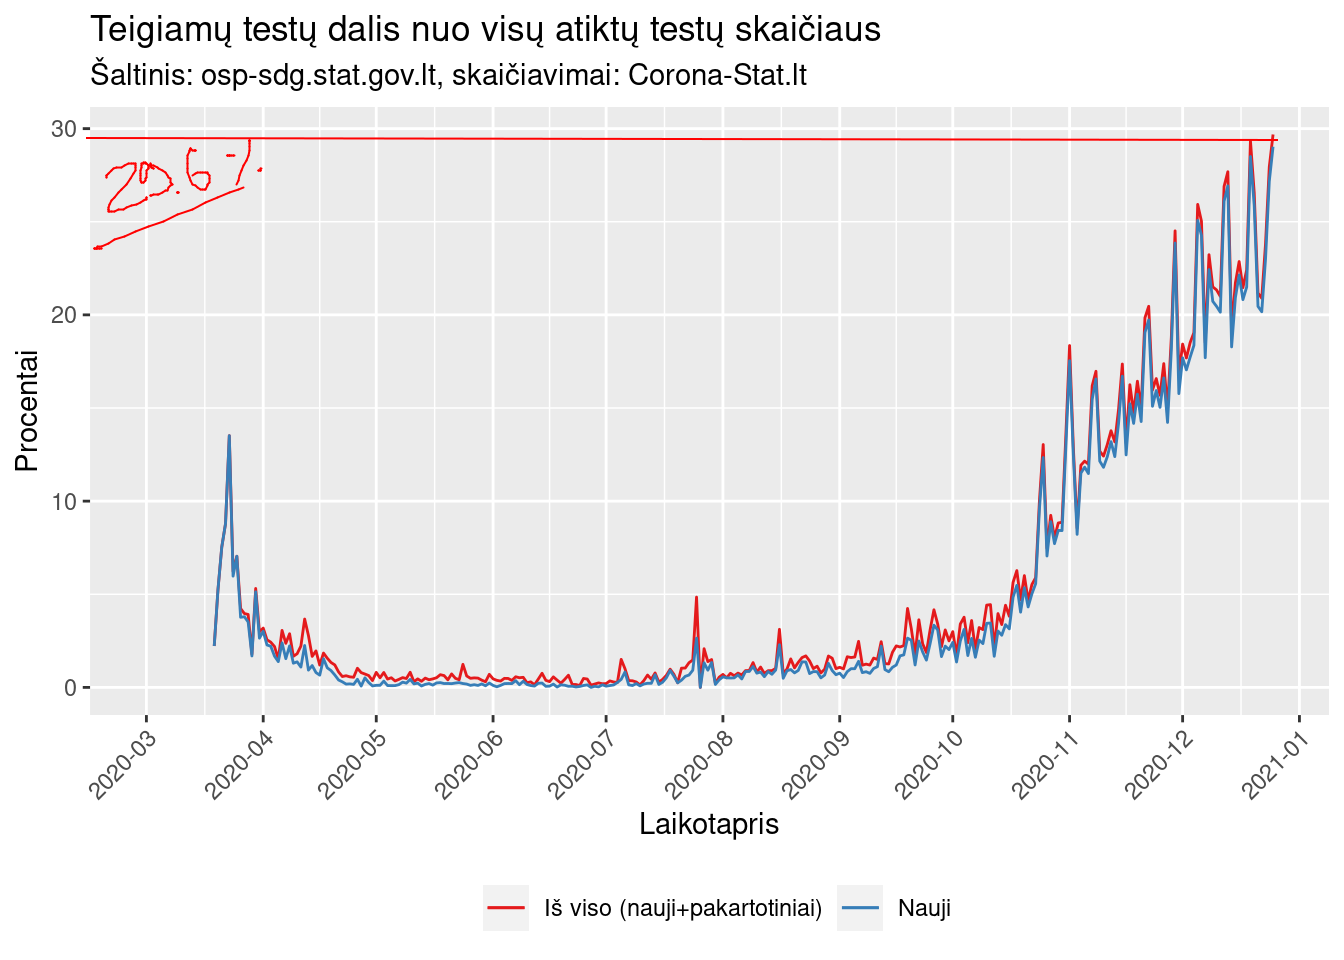
\includegraphics[width=0.1\textwidth]{1.png}

Lietuvos medikų sąjūdžio valdybos pirmininkė Živilė Gudlevičienė 

\includegraphics[width=0.1\textwidth]{5.png}

Lietuvos profesinės sąjungos “Solidarumas” gen. sekretorius Ričardas Garuolis

\includegraphics[width=0.1\textwidth]{6.png}

Lietuvos švietimo darbuotojų profesinės sąjungos pirmininkas Andrius Navickas
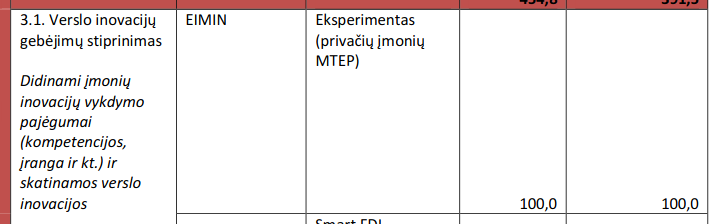
\includegraphics[width=0.15\textwidth]{3.png}

Lithuanian-Economy.net ekonomistas Justas Mundeikis

\includegraphics[width=0.1\textwidth]{2.png}

VU Filosofijos fakulteto profesinės sąjungos pirmininkė Rūta Žiliukaitė
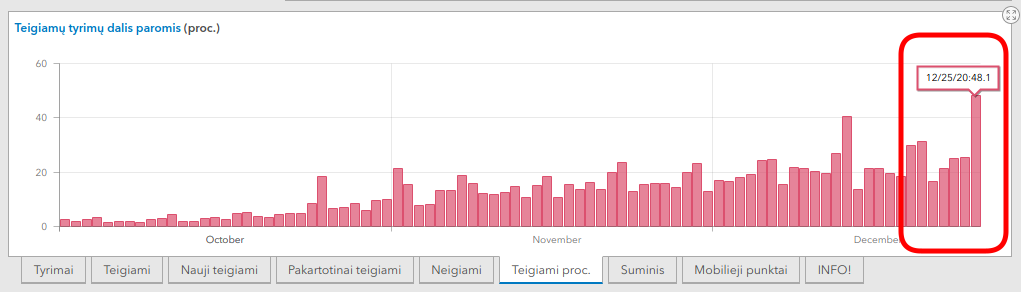
\includegraphics[width=0.15\textwidth]{4.png}



\end{document}
